\documentclass[senior,final,11pt]{iscs-thesis}
\usepackage[dvipdfmx]{graphicx}
\etitle{A Method of Improving QoS:  Explorations of the Possibility of Function Combinations in Service Compositions}
\jtitle{品質改良のアプローチ:機能のぶれを許すサービス合成}
%
\eauthor{Ziyuan Wang}
\jauthor{王子源}
\esupervisor{Shinichi Honiden}
\jsupervisor{本位田真一}
\supervisortitle{Professor} % Professor, etc.
\date{February 9, 2016}
%-------------------
\begin{document}
\begin{eabstract}
There is a growing need for web service providers to develop customised and flexible web services as quick as they can. One way to satisfy this demand is to utilise service compositions, which provide a method of consolidating several services to a richer service. Because of the uncertainty in the feasibility of the functional and QoS requirements, it is not guaranteed that service compositions succeed with suitable solutions.

One way to satisfy the given requirements is to control the given two kinds of requirements. There have been studies on methods of optimising the QoS with fixed functional requirements. However, the search space in that case is limited, which would possibly not include service compositions with better QoS whose functions are slightly different from the required one. Therefore, I focus on the possibility of improving the QoS by compromising on functions or exploring the possibility of function combinations. This enables better advice of service compositions to users. In this article, I propose a method of efficiently searching different possibilities to support users to balance functional requirements and QoS requirements.
\end{eabstract}
\begin{jabstract}
近年,ウェブサービスプロバイダーにとって,ユーザーの好みに合わせた,柔軟なウェブサービスを短時間で作る必要性が増してきている.そのために,よく使われている手法として,複数のサービスを一つにまとめてより高機能なサービスを作るサービス合成と呼ばれる手法がある.サービス合成において,入力として受け取る機能や品質に関する要求を必ず満たせるとは限らないという問題がある.

機能と品質の両方を達成するために既存研究で提案されている手法として,その片方を固定して保証し,もう片方を最適化するというものがある.しかし,この手法では,機能を固定するために,探索空間が限られているため,
要求された機能に妥協を許した場合に品質が大きく高まるような合成を見逃す可能性がある.よって,本論文では,ユーザーが高品質の合成を見つけることがより容易になるよう,機能を妥協し,要求された機能と少しのぶれを許すことで探索空間を増やすことによるQoSの最適化の可能性について議論した.本論文では,ユーザーが機能要求と品質要求のバランスを取れるように効率的に様々な合成の可能性を探索する手法を提案した.

\end{jabstract}
\maketitle

\begin{acknowledge}
I appreciate Prof. Ishikawa's help in improving the structure of the paper.
\end{acknowledge}

\frontmatter 
\tableofcontents
%\listoffigures
%\listoftables 
%\lstlistoflistings
%-------------------
\mainmatter 

\chapter{INTREODUCTION}
Web service, service-based system, and service composition are significant.
%ws 基于service的系\UTF{7EDF} 和service合成是很重要的
A lot of existing studies on QoS-aware service composition.
%介\UTF{7ECD}下上面提到的几个名\UTF{8BCD},\UTF{8BA8}\UTF{8BBA}下它\UTF{4EEC}的来\UTF{9F99}去脉 
Fixed functional requirements -> may lose potential improvement of QoS, difficulty for users to properly define the functional requirements because of uncertainty of the feasibility of requirements given available services
%\UTF{8BA8}\UTF{8BBA}它\UTF{4EEC}的不好,固定fun\UTF{5BFC}致没法找到更好的qos
Tis paper ... (summary of the remainder).
%本文的主\UTF{9898},干了什\UTF{4E48}。
Chapter 2 describes ... Chapter 3...
%\UTF{6BCF}一章做了什\UTF{4E48}%
\section{Background}
%背景
\section{Goals}
%我\UTF{4EEC}的目的
\section{Contributions}
%本文的\UTF{8D21}献
\cite{4065825}. 
%-------------------
\chapter{Preliminary}%1-18------------------------
%已有的定\UTF{4E49}%
%Existing definitions.
~~~~This section defines some key terms of formal research of the service composition that I continue to use in this paper.
\section{Service}
%所\UTF{8C13}service,就是功能可重\UTF{590D}利用的
~~~~A service S is a reusable system that provides functionalities which are documented in a service description. This description defines a 5-tuple {\em IOPEQ = (S.I, S.O, S.P, S.E, S.Q)} where {\em S.I, S.O} are abbreviated from the required inputs and outputs of the S, {\em S.P, S.E} are the preconditions and effects which denote the necessary condition of utilising S and the consequence after running S, and {\em S.Q} is the set of the QoS attributes of the S. \\
%\UTF{5173}于service,一般分成service(instance)和service task\UTF{4E24}\UTF{79CD}\UTF{8BF4}法。service task
~~~~In this paper, {\em S.P, S.E} are ignored therefore a service S is modelled only with 3-tuple {\em IOQ = (S.I, S.O, S.Q)}.
%service (instance) and service task
%IOPEs -> modelled only with IO in this paper
%+ 
%Q
\section{QoS}
~~~~QoS is abbreviated from quality-of-service, that is, quality apart from the functionality the service can provides, such as the price, the execution time and the reliability of the service.
The S.Q of a service S is consist of a number of QoS attributes which is normalized between 0 and 1, with 0 being the worst and 1 being the best.
%multi-criteria
%normalized

\section{Service Compliance}
%Connectivity between two services
~~~~If there exists an output {\em o} $\in$ {\em S.O} of a service S is compatible with an input of {\em i}  $\in$ {\em S'.I} of another service S', we say there is a service link between S and S', written as S $\to$ S'. That is, the type of {\em o} is the same or a subtype of i. \\
~~~~In this paper, a service is constrained to has only one input and one output, therefore S $\to$ S' iff:
\begin{center}
{\em o} = {\em S.O} ,  {\em i} = {\em S'.I} ,  {\em o} $\in$ {\em i}
\end{center}

\section{I/O Plug-in match}
%我\UTF{4EEC}可以根据input或者output的兼容\UTF{5173}系来\UTF{7ED9}\UTF{4E24}个差不多功能的
~~~~Two functionality similar services, in this paper that denotes they are in the same task, may have two relations, defined as follow.\\
~~~~An Input Plug-in match $\sqsubseteq$ is a S $\times$ S relation that holds iff:
\begin{center}
S $\sqsubseteq$ S'  $\Leftrightarrow$ {\em S.I} $\in$ {\em S'.I}
\end{center}
~~~~In this paper, S $\sqsubseteq$ S' is referred to as S' is input-stronger than S, and S is input-weaker than S'.\\
~~~~An Output Plug-in match $\subset$ is a S $\times$ S relation that holds iff:
\begin{center}
S $\subset$ S' $\Leftrightarrow$ {\em S.I} $\in$ {\em S'.I}
\end{center}

In this paper, S $\subset$ S' is referred to as S' is output-stronger than S, and S is output-weaker than S'.\\

\section{Functional requirements}
%用\UTF{6237}想要合成的大service的 功能,也就是\UTF{8F93}入type和\UTF{8F93}出type

\section{Workflow}
~~~~A workflow is a sequence of two or more linked services. The functions of a workflow depend on function combinations that consist of the input parameter of the workflow's first service and the output parameter of the workflow's last service. A workflow template contains service tasks instead of actual services. A task is characterised as an abstract functionality which can be replaced by an actual service. There are generally two ways to assign services to a task, one is to compare the functions of the services with the functional requirements of the task. The other is to collect services depend on documents such as service description, which are usually distributed with the service by provider. Finally, each task is assigned with a set of services which meet the functional requirements of the task.

Selection algorithms receive a workflow template with fixed functional requirement and a dozens of services, and select for each task of one or more services which guarantee the obtained workflow's QoS are optimised, then return the obtained workflow as an output.

%Figure 1 shows an example workflow template and a possible service selection. may be add after
%Functional requirements: ぶれなし (existing)


\section{QoS optimization}%有空找找看\UTF{7C7B}似的。\UTF{8BF4}好我\UTF{4EEC}\UTF{8FD9}里是不考\UTF{8651}QoS限制的
%this time single-objective
\section{Service composition}
%我用一下式子給service composition\UTF{8FDB}行一个原始的定\UTF{4E49}:
%input:固定的workflow template 一群service, function requirements,output:最\UTF{4F18}的workflow
\chapter{Related  work}
%今天决定要写几个,可以从之前的\UTF{8BBA}文中\UTF{9009} 1000字


%-------------------
\chapter{Approach}%1-20
%(\UTF{8FD9}里\UTF{641E}点\UTF{56FE}\UTF{554A})。我的approach被\UTF{56FE}?表示出来。
%我\UTF{4EEC}在下一个section中介\UTF{7ECD}了\UTF{8FD9}\UTF{6837}paper主要研究的\UTF{95EE}\UTF{9898}的定\UTF{4E49}(\UTF{56FE})。
%在第二个section我\UTF{4EEC}介\UTF{7ECD}了解决上述\UTF{95EE}\UTF{9898}的具体算法。第一,我\UTF{4EEC}在section??中先解\UTF{91CA}下如何将\UTF{6BCF}一个task中的service\UTF{4EEC}clustering化。clustering化的好\UTF{5904}有\UTF{5565}?clustering之后,相\UTF{5BF9}于一\UTF{5F20}task就能有一\UTF{5F20}“地\UTF{56FE}”,可以在之后的skyline算法的\UTF{65F6}候参照它利用它。第二,我\UTF{4EEC}在subsection??中介\UTF{7ECD}了skyline的算法。比起用全探索,skyline算法可以有效地\UTF{51CF}少\UTF{8BA1}算量,\UTF{8FD9}\UTF{8BA9}整个系\UTF{7EDF}的可行性大大\UTF{589E}加,我\UTF{4EEC}之后的\UTF{8BA1}算都是基于skyline算法的。第三,我\UTF{4EEC}在第subsection??中介\UTF{7ECD}了naive algorithm,它在skyline算法的基\UTF{7840}上,\UTF{7B80}\UTF{5355}地将9\UTF{79CD}可能的bure情况分\UTF{522B}\UTF{8FD0}算,然后根据得到的9个\UTF{7ED3}果,互相比\UTF{8F83}之后得出最好的\UTF{7ED3}果后\UTF{7ED9}用\UTF{6237}\UTF{8FDB}行推荐。第四,我\UTF{4EEC}在subsection??中介\UTF{7ECD}了development algorithm,它在naive的基\UTF{7840}上改\UTF{8FDB}了算法,\UTF{7B80}\UTF{5355}来\UTF{8BF4},根据是否\UTF{62E5}有相同\UTF{5F00}\UTF{5934}来将9\UTF{79CD}可能分成3\UTF{7EC4},一\UTF{7EC4}3\UTF{79CD}可能。比起naive algorithm,它也有效地\UTF{51CF}少了\UTF{8BA1}算量

\section{Extended Composition Problem}: Proposal1 %1-20 bure\UTF{95EE}\UTF{9898}的定\UTF{4E49}%
%就如同我之前在section。。所提到的,由于 能否\UTF{6EE1}足funcitonal requirements\UTF{8FD9}件事并不是那\UTF{4E48}明\UTF{663E}  所以\UTF{4E25}格将用\UTF{6237}所提出的funcitonal requirements作\UTF{4E3A}service composition system的\UTF{8F93}入的\UTF{8BDD},会存在\UTF{6EE1}足功能的workflow不存在,或者是 由于探索空\UTF{95F4}的不足而\UTF{5BFC}致找不到真正最\UTF{4F18}qos的workflow的情况出\UTF{73B0}。我\UTF{4EEC}\UTF{9488}\UTF{5BF9}\UTF{8FD9}个\UTF{95EE}\UTF{9898},提出了不\UTF{4EC5}探索fixed functional requirements,并且同\UTF{65F6}探索它的Bure 的解决方案。我\UTF{4EEC}首先引\UTF{8FDB}以下的定\UTF{4E49}%

%%%\UTF{8FD9}段不用翻\UTF{8BD1}%
%参照chapter2。。
%\UTF{5BF9}于一个start service 它的Strong 集合 是在同一task中input stronger than it(但是不包含自己)
%\UTF{5BF9}于一个start service 它的Weak集合是 在同一task中input weaker than it(但是不包含自己)。特\UTF{522B}的,one_weak集合是指,Weak中的 start service相\UTF{8FDE}接 的subset
%\UTF{5BF9}于一个end service 它的Strong 集合 是在同一task中output stronger than it(但是不包含自己)
%\UTF{5BF9}于一个end service 它的Weak集合是 在同一task中ouput weaker than it(但是不包含自己)。特\UTF{522B}的,one_weak集合是指,Weak中的 end service相\UTF{8FDE}接 的subset
%\UTF{5BF9}于一群start或者end services的集合 \UTF{8FD9}个集合的Strong集合就是各个service的strong集合的并集,\UTF{8FD9}个集合的weak集合就是各个service的one_weak集合的并集(但是不包含自己)
%%%\UTF{8FD9}段不用翻\UTF{8BD1}%

%在QoS不降低的情况下提高多少程度的功能都是很\UTF{4E50}意被人看到的(be expected),但是如果qos提高是以功能的\UTF{51CF}弱\UTF{4E3A}代价的\UTF{8BDD},那\UTF{4E48}\UTF{51CF}弱的程度必\UTF{987B}要有个限制(actually, not so meaningful to use too weak services)。this paper中,我\UTF{4EEC}只取功能降低一段(隣接)的weak,将功能的\UTF{51CF}弱控制在\UTF{8F83}低范\UTF{56F4}。
%我\UTF{4EEC}\UTF{7EE7}\UTF{7EED}定\UTF{4E49}start/end services的bure:
%bure:\UTF{5BF9}于一个fixed集合,它的Strong和one_weak和它自己的tuple定\UTF{4E49}\UTF{4E3A}bure(定\UTF{4E49})
%接下来我\UTF{4EEC}定\UTF{4E49}bure\UTF{95EE}\UTF{9898}:
%\UTF{5BF9}于functional requirement = (fixed_start, fixed_end),我\UTF{4EEC}不\UTF{4EC5}\UTF{4EC5}在原来的\UTF{95EE}\UTF{9898}\UTF{8BBE}定的基\UTF{7840}上(参考service composition)\UTF{8BA1}算它,\UTF{8FD8}\UTF{8BA1}算以start_bure  * end_bure \UTF{4E3A}\UTF{5934}尾的function 的9\UTF{79CD}function中的剩余8\UTF{79CD}。然后\UTF{8F93}出(fixed,fixed)和 剩下8\UTF{79CD}中比它QoS高的



%motivation again

%ぶれありのcomposition problem定義
%def. 何段階ずれてもよい
%(actually, not so meaningful to use too weak services)


\section{Algorithm for Extended Composition Problem}: Proposal 2%1-20 bure\UTF{95EE}\UTF{9898}的具体算法
%我\UTF{4EEC}在\UTF{8FD9}个section中\UTF{8BF4}明\UTF{8FD9}\UTF{4E48}具体地,一\UTF{6B65}\UTF{6B65}地解决上面的\UTF{95EE}\UTF{9898}%
\subsection{Functionality Graph}%\UTF{9636}\UTF{5C42}化
%From [Wagner'11]
%def.
%algorithm
%在[Wagner'11]中,它定\UTF{4E49}了functionality graph。如何\UTF{8BA1}算functional graph:将同一task中的services做\UTF{4E3A}\UTF{8F93}入,根据他\UTF{4EEC}之\UTF{95F4}的output的service Compliance\UTF{5173}系 ,(\UTF{8FD9}里改写下,直接英\UTF{8BED})插入\UTF{4E24}\UTF{5F20}\UTF{56FE}(\UTF{4F2A}代\UTF{7801}可有可无,写\UTF{4F2A}代\UTF{7801}太\UTF{70E6}了)
%


\subsection{Skyline}%skyline 算是准\UTF{5907}工作
%def.
%algorithm
%算法的意\UTF{4E49},吃了什\UTF{4E48}吐了什\UTF{4E48}(文字):
%算法\UTF{4F2A}代\UTF{7801}:(先用手写)
%算法的\UTF{8BF4}明

\subsection{Naive Algorithm}%naive
%能写的\UTF{5E94}\UTF{8BE5}不多,input output 重申一下(注意 \UTF{8FD9}里的output是“方案”),吐槽一下怎\UTF{4E48}怎\UTF{4E48}不行就走
%for all 機能のぶれ (same, IN_one_weak-OUT_same, IN_same-OUT_one_weak, ...)
 % solve

\subsection{Developed Algorithm}%\UTF{641E}个牛逼的名字
%bure算法是基于naive算法的改\UTF{8FDB}算法。
%\UTF{8865}上算法1-22写 1-21日已\UTF{7ECF}没\UTF{8111}子了



\chapter{Experiments}
%在\UTF{8FD9}一章,我\UTF{4EEC}主要介\UTF{7ECD}我\UTF{4EEC}的\UTF{5B9E}\UTF{9645}做的\UTF{5B9E}\UTF{9A8C}。
%第一\UTF{8282}介\UTF{7ECD}了\UTF{5B9E}\UTF{9645}的\UTF{8FD0}行\UTF{73AF}境 和 具体的\UTF{8FD0}行\UTF{573A}景(10task10service,random QoS。random input output requirements . random input output compliance)
%第二\UTF{8282}介\UTF{7ECD}了由bure\UTF{95EE}\UTF{9898}的\UTF{8BBE}定所能\UTF{5E26}来的好\UTF{5904}。介\UTF{7ECD}了\UTF{8BD5}\UTF{9A8C}方法并\UTF{8BC4}价了好\UTF{5904}的大小
%第三\UTF{8282}介\UTF{7ECD}了\UTF{4E3A}了高速化我做出的\UTF{4E24}次功夫。并且通\UTF{8FC7}\UTF{5BF9}比step数 \UTF{8BC4}价了\UTF{6BCF}次\UTF{4F18}化快了多少。
\section{Implementation}
Implemented with Python.
%本\UTF{5B9E}\UTF{9A8C}的実装部分的\UTF{73AF}境是python2.7。\UTF{8BC4}价部分的\UTF{73AF}境是R 3.2.3\UTF{6267}行的。
%具体的基本\UTF{8BBE}定:正如同之前的prelimiar中所介\UTF{7ECD}的,是基于service composition中的selection 方法的\UTF{8BBE}定的。在\UTF{8FD9}里,我将work flow template \UTF{8BBE}定成由10个\UTF{5934}尾相接(1条直\UTF{7EBF}没有分支,一个output\UTF{5BF9}\UTF{5E94}着1个input)的task\UTF{7EC4}成,\UTF{6BCF}个task\UTF{62E5}有不同function不同qos的10个service。\UTF{6BCF}个service的qos都是由十个0到1之\UTF{95F4}的数\UTF{7EC4}\UTF{6784}成的vector\UTF{7EC4}成的。
%怎\UTF{4E48}\UTF{5B9E}\UTF{9645}操作S.I S.O......,可以参考2012年的\UTF{8BBA}文(\UTF{5B9E}在不行可以修改之前的\UTF{8BBE}定)。由于考\UTF{8651}S.I S.O具体到底代表什\UTF{4E48}很耗\UTF{65F6}\UTF{95F4}并且并不是我\UTF{4EEC}\UTF{95EE}\UTF{9898}的核心,所以我\UTF{4EEC}直接考\UTF{8651}service之\UTF{95F4}的\UTF{8FDE}接情况。
%\UTF{5BF9}于\UTF{6BCF}个service能\UTF{591F}\UTF{8FDE}接的下一个task中的service就是随机的,。\UTF{8FD9}\UTF{6837}可以解决除了start_task的input 的 end_task的output中的\UTF{9636}\UTF{7EA7}\UTF{5173}系  之外的\UTF{9636}\UTF{7EA7}\UTF{5173}系,\UTF{786E}定了除了start_task的  和end_task之外所有service的\UTF{8FDE}接情况。(因\UTF{4E3A}没有\UTF{8FDE}接到start_task的  和end_task能\UTF{8FDE}接的 service  的存在)。\UTF{8FD9}里\UTF{5BF9}于\UTF{8FD9}里的\UTF{9636}\UTF{7EA7}\UTF{5173}系的“\UTF{5F3A}弱”的界定并不是本文所\UTF{5173}心的,所以\UTF{5BF9}于start_task的input 的 end_task的output中的\UTF{9636}\UTF{7EA7}\UTF{5173}系也是随机决定的。决定方法如下:在本文中 ,\UTF{4E3A}了\UTF{8BBE}定方便, \UTF{53E6}外在start_task的之前和end_task之后\UTF{4F2A}造了\UTF{4E24}个task,根据他\UTF{4EEC}之\UTF{95F4}的\UTF{8FDE}接\UTF{5173}系\UTF{786E}定了 start_task的input 的 end_task的output中的\UTF{9636}\UTF{7EA7}\UTF{5173}系。一般\UTF{8BA4}\UTF{4E3A}input的\UTF{5F3A}指 可以接受的type多, output的\UTF{5F3A}指可以\UTF{8F93}出的type的多,反之\UTF{5219}弱。(\UTF{4E3E}个例子,input的“可以接受jpg和png”比“只可以接受jpg”要\UTF{5F3A}。output的“可以\UTF{8F93}出mp3或者mp4”比“只可以\UTF{8F93}出mp3”要\UTF{5F3A},反之依然),其\UTF{5B9E}如同在prelimiar中提到的,\UTF{8FD8}可以参考文档之列的解决方法,但我就是任性不用。不爽去看2012年的\UTF{8BBA}文。

\section{Extended Composition Problem}
Evaluation of Proposal 1\\
How QoS can be improved by allowing compromise in functional requirements?
%\UTF{8FD9}个\UTF{8BD5}\UTF{9A8C}的目的:How QoS can be improved by allowing compromise in functional requirements?
%\UTF{8BC4}价\UTF{8BD5}\UTF{9A8C}\UTF{8BBE}\UTF{8BA1}:\UTF{8BA1}算了1000回(\UTF{8FD9}里\UTF{5BF9}回要有定\UTF{4E49}:将input集\UTF{9F50},投入system\UTF{8FDB}行一次\UTF{8BA1}算叫做回,定\UTF{4E49}在service composition中),\UTF{5BF9}比\UTF{5BF9}象 1\UTF{8BA1}算固定functional requiments所得出的qos  2  9\UTF{79CD}不同情况的bure function下的qos。
%得出的\UTF{7ED3}果如下\UTF{56FE}所示(\UTF{56FE}表)。#我\UTF{4EEC}可以看到8\UTF{79CD}情况的表\UTF{73B0}。\UTF{8FD9}\UTF{6837}看可能不直\UTF{89C2}。(可能不要,没多大用)

%(考\UTF{8651}将\UTF{8FD9}个定\UTF{4E49}放在之前)如何\UTF{8BC4}价方案的好坏:将方案的所有“\UTF{9009}\UTF{62E9}” 比起fixed的改\UTF{8FDB}比例 相加,\UTF{8FD9}个数\UTF{503C}越高方案越好。

%我\UTF{4EEC}根据\UTF{5BF9}bure的function的容忍程度 \UTF{8FDB}一\UTF{6B65}\UTF{5BF9}8\UTF{7EC4}的情况\UTF{8FDB}行情况的分\UTF{7C7B}。
%第一\UTF{79CD}情况:只允\UTF{8BB8}\UTF{4E25}格意\UTF{4E49}上功能\UTF{589E}\UTF{5F3A}的bure集合。也就是只承\UTF{8BA4}(s,s),(s,f),(f,s)\UTF{8FD9}3\UTF{79CD}%
%第二\UTF{79CD}情况:广\UTF{4E49}上功能\UTF{589E}\UTF{5F3A}的bure集合。比上面多承\UTF{8BA4}(s,o),(o,s)
%第三\UTF{79CD}情况:允\UTF{8BB8}功能\UTF{51CF}弱的bure集合。比上面多承\UTF{8BA4}(o,o),(o,f),(f,o)
%\UTF{8FD9}也可放前面介\UTF{7ECD}%

%我\UTF{4EEC}看下 3\UTF{79CD}不同bure的表\UTF{73B0}。(插入\UTF{56FE})
%可以看\UTF{89C1}随着\UTF{5BF9}bure的程度的容忍度 \UTF{589E}加,越容易得到改\UTF{8FDB}方案,并且改\UTF{8FDB}方案的\UTF{8D28}量也会\UTF{589E}加。




\[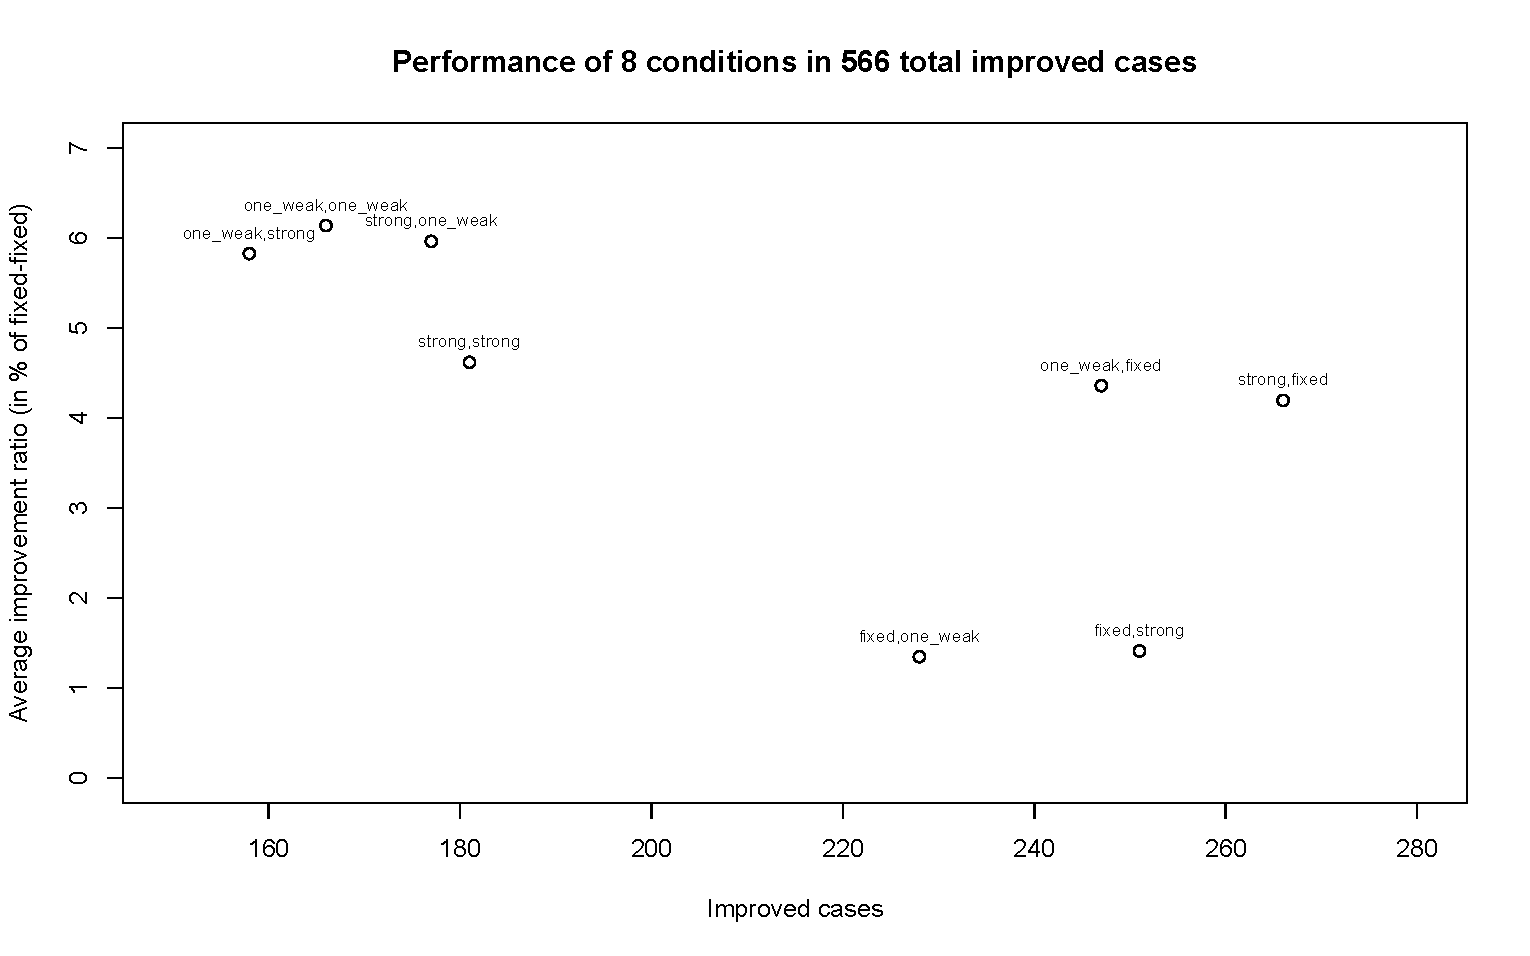
\includegraphics[width=13cm]{eval2.pdf}\]

\section{Algorithm}
Evaluation of Proposal 2\\
How fast can the proposed algorithm solve the extended problem?\\
- with skyline vs. without skyline\\
Fig. x depicts the relationship of step numbers between full search and skyline algorithm.
\[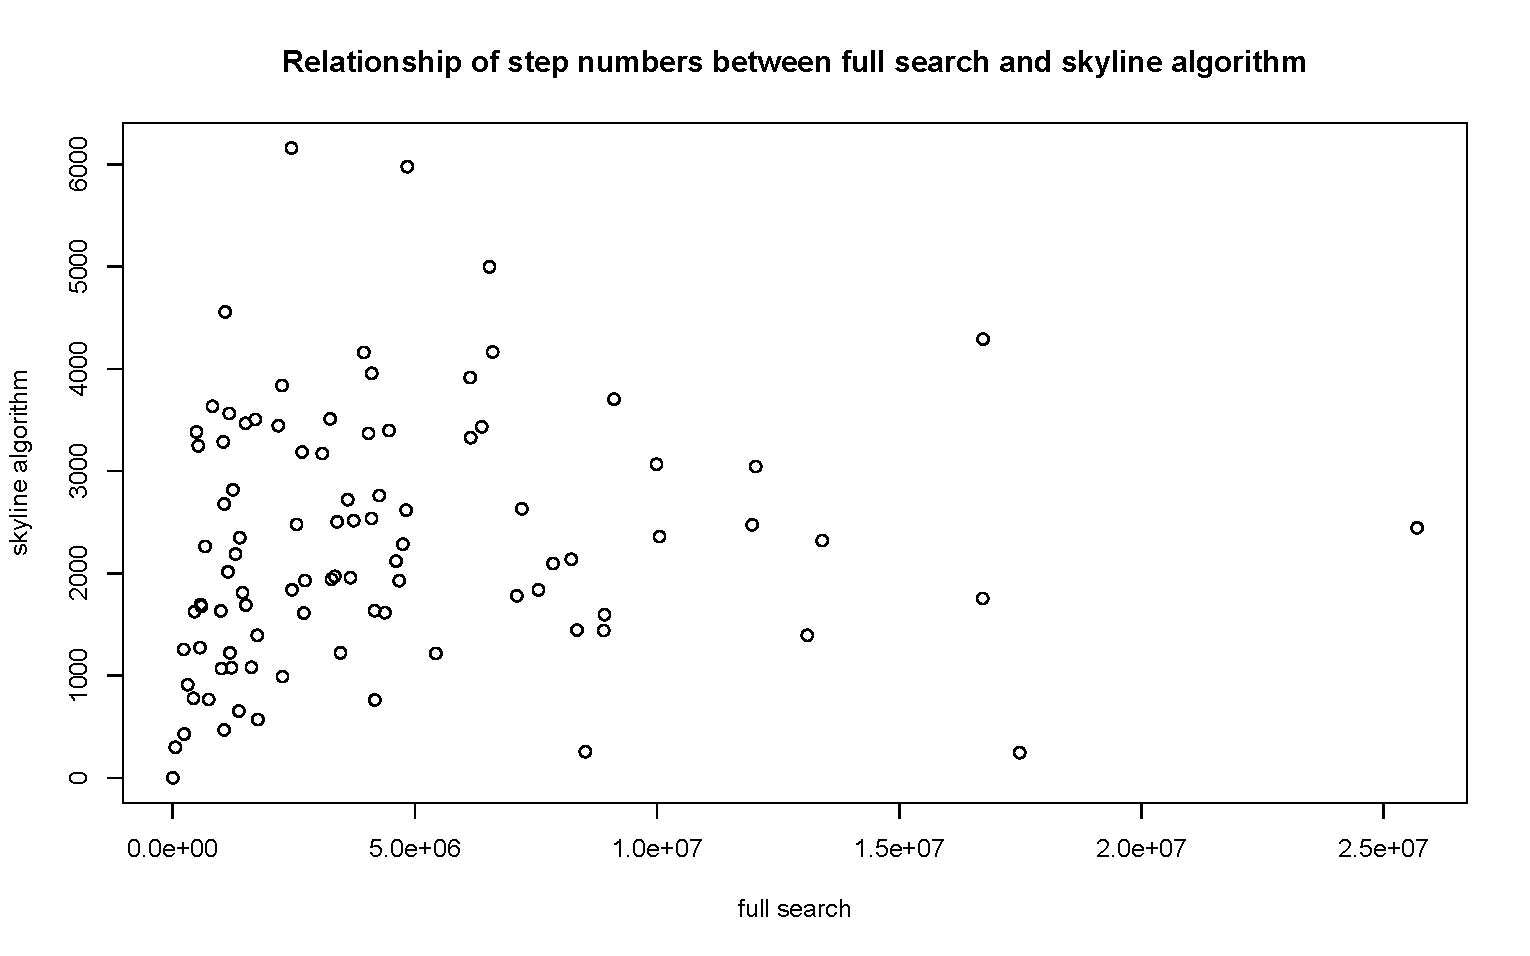
\includegraphics[width=13cm]{eval1.pdf}\]
By further calculation, the correlation between them is measured to be 0.1814083, which demonstrate the existence of weak correlation.\\
%我\UTF{4EEC}可以看到step numbers 降到1/1992,(再加一个\UTF{65F6}\UTF{95F4}\UTF{56FE})。
%further eval:有\UTF{4E24}个\UTF{53D8}量。task数和workflow数(算了 之后再考\UTF{8651} 估\UTF{8BA1}没\UTF{65F6}\UTF{95F4}。2月\UTF{4EFD}做\UTF{5427})
%全探索的探索空\UTF{95F4}是task内的services数 的 task\UTF{603B}数次方。
%skyline之后的探索空\UTF{95F4}是(skyline之后的task内的services数)。。有点算不出来。要\UTF{8BBE}\UTF{8BA1}\UTF{5B9E}\UTF{9A8C}的\UTF{8BDD}:1 保持task数不\UTF{53D8} \UTF{589E}加\UTF{6BCF}个task内的services数 2 保持task内的service不\UTF{53D8},\UTF{589E}加task的\UTF{603B}数

- with skyline vs. proposed algorithm with skyline
%\UTF{8FD9}里想\UTF{529E}法\UTF{7F29}成一幅\UTF{56FE}。或者按照老\UTF{5E08}的\UTF{8BF4}法 做成worst best average\UTF{56FE}。无\UTF{8BBA}如何 算一个\UTF{65F6}\UTF{95F4}\UTF{5427}。(将写写入去掉 只\UTF{8BA1}算\UTF{65F6}\UTF{95F4}(将\UTF{65F6}\UTF{95F4}\UTF{8F93}出到csv中 ),今天\UTF{665A}上\UTF{8DD1})
\[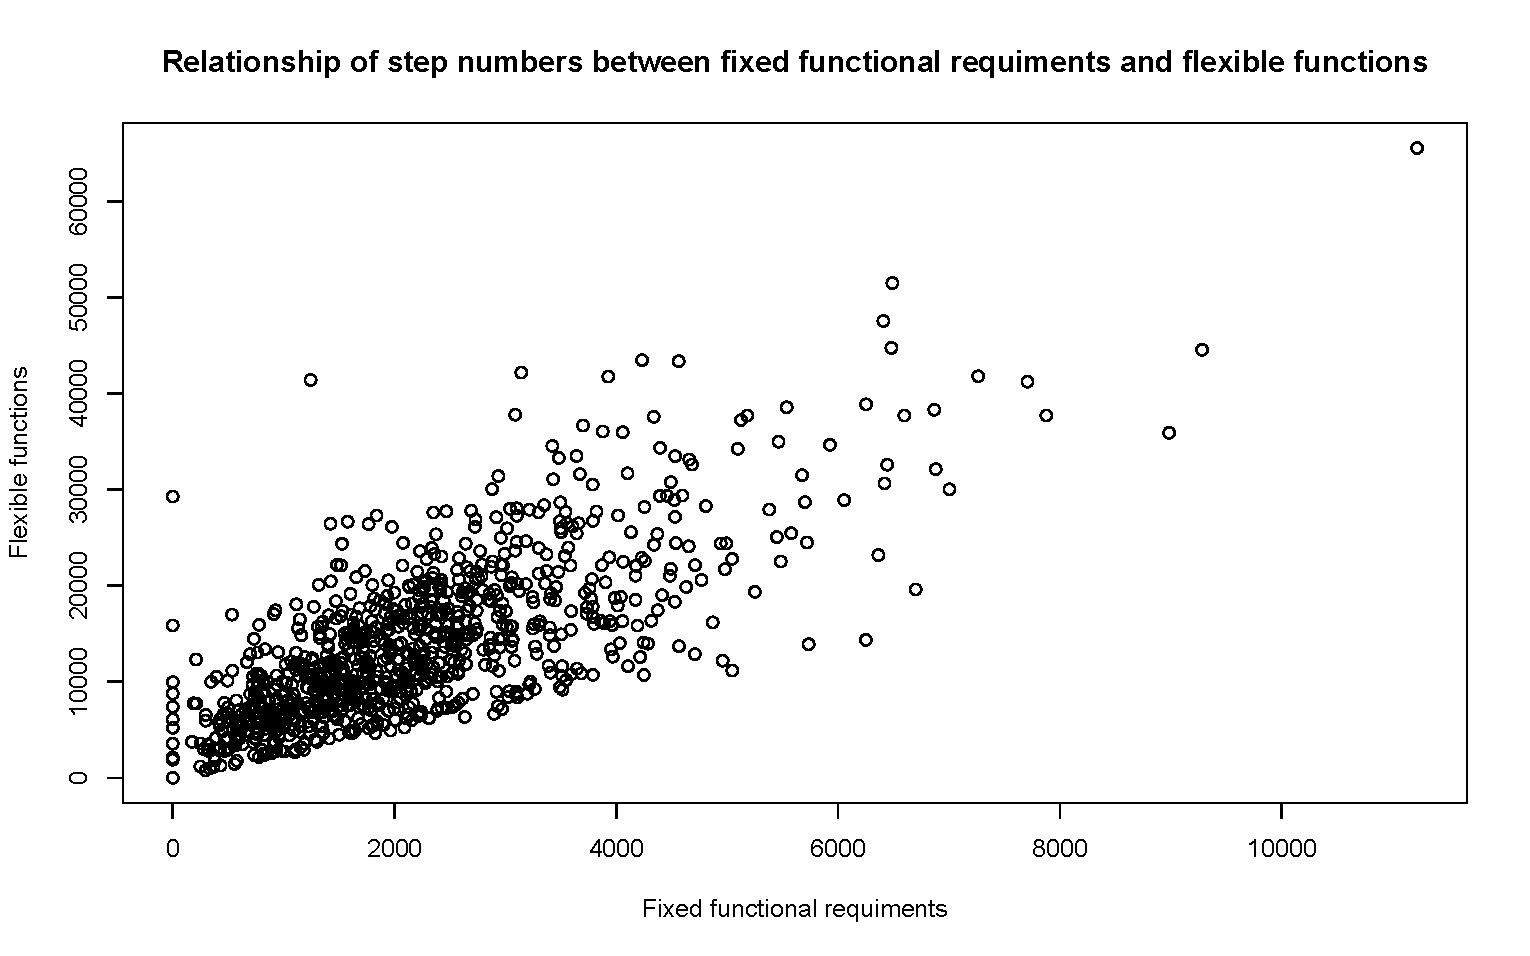
\includegraphics[width=13cm]{eval3-1.pdf}\]
\[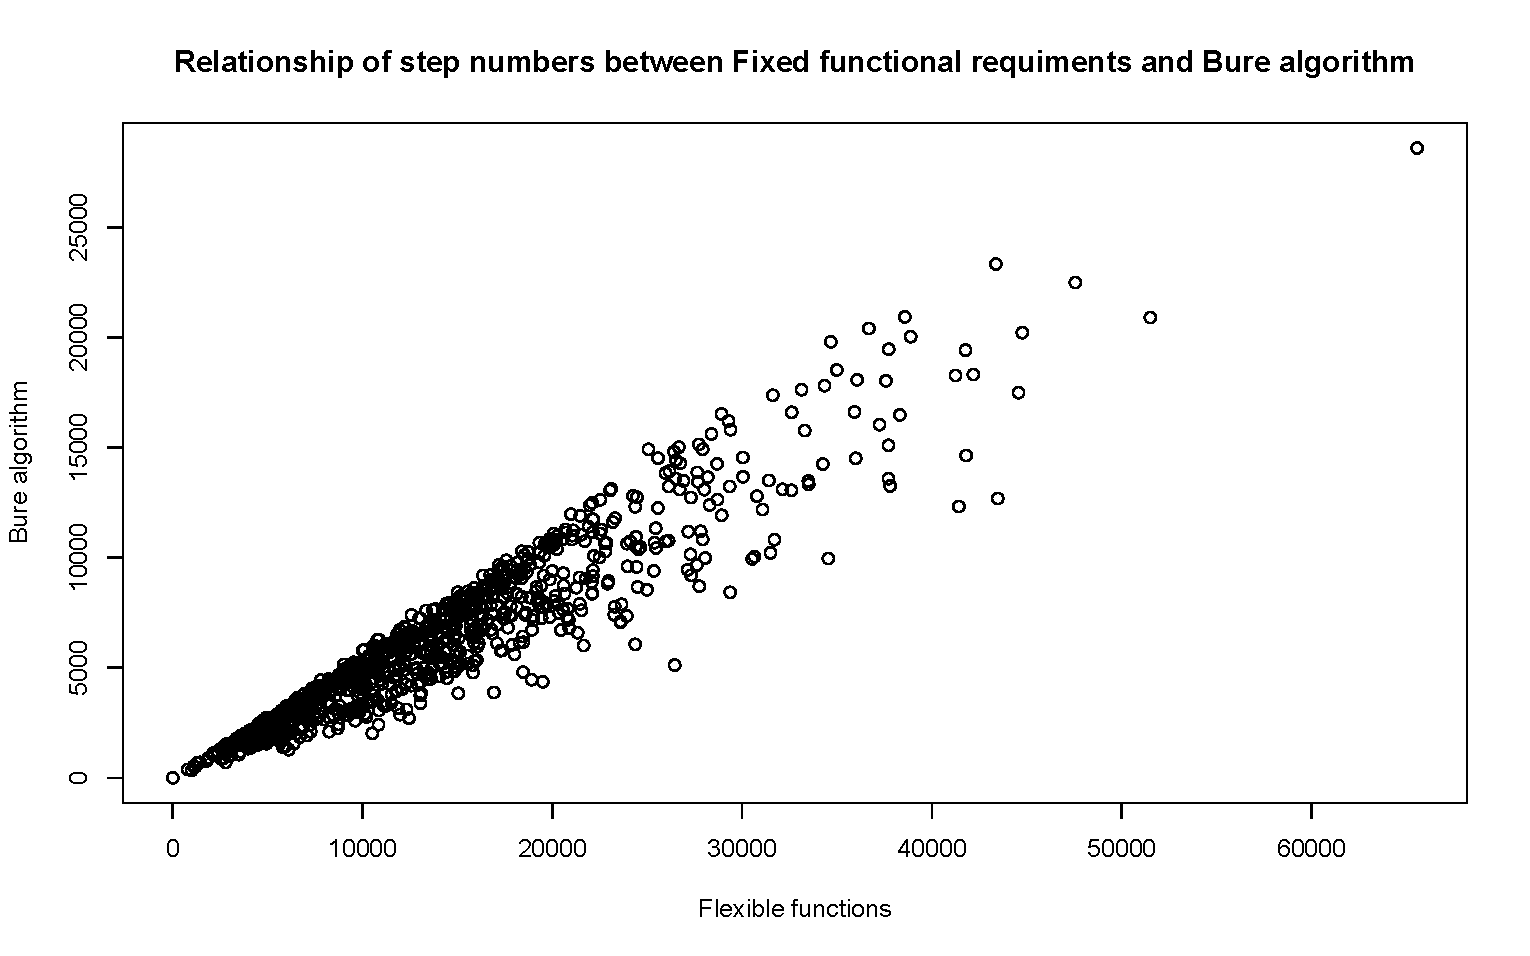
\includegraphics[width=13cm]{eval3-2.pdf}\]
\[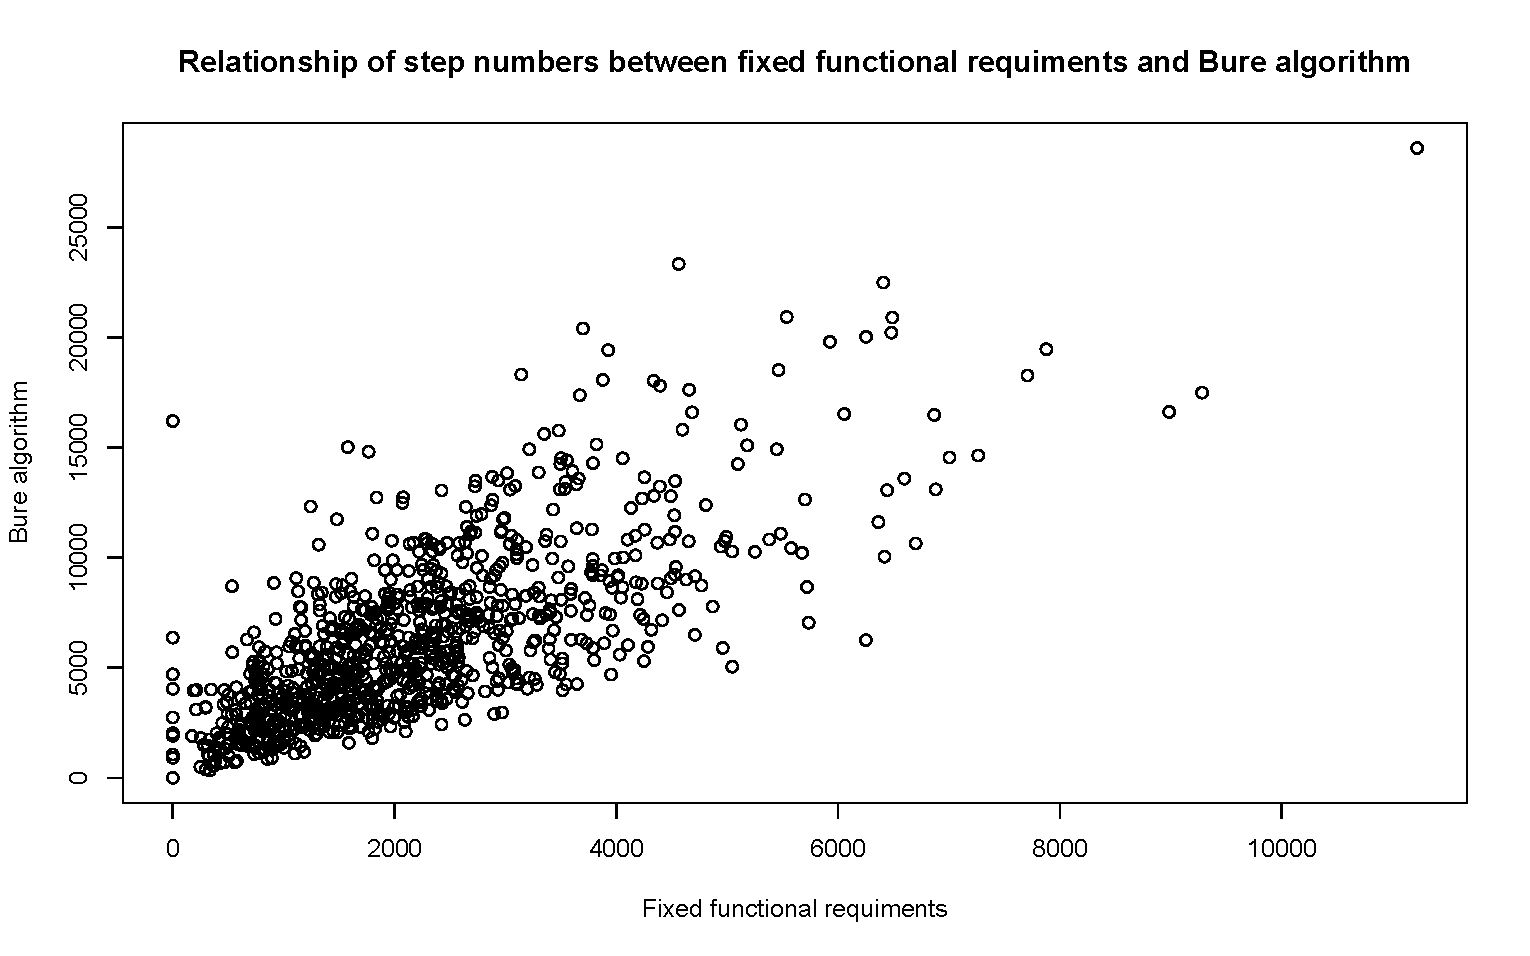
\includegraphics[width=13cm]{eval3-3.pdf}\]

\chapter{Discussion}
% related work can come here

\subsection{Proposal}
The extended problem should be significant because in the experiment

The proposed algorithm made good improvement because in the experiment 

% if difficult, combine to the experiment chapter

\subsection{Future Work}
- QoS constraints
- adaptive


\chapter{Conclusion}

%-------------------
\bibliographystyle{plain} 
\bibliography{myref} 
%-------------------
\end{document}
